\section{Problemstilling}
Reinseanlegget er teknisk utdatert og treng forbetring. Styringssystemet, som no er over tjue år gammalt,
består hovudsakeleg av eldre og utgåtte komponentar. Med eldre komponentar aukar risikoen for svikt, 
og det kan vere vanskeleg å finne passande reservedelar.

WaterCare AS\citep{WaterCare}, som opphavleg leverte styresystemet har i seinare tid blitt avvikla. Dette gjer at kompetansen 
og moglegheita for å gjere endringar i styresystemet er utfordrande. 
På grunn av desse utfordringane har ikkje anlegget klart å halde tritt med den teknologiske utviklinga, 
og mindre problem har gradvis bygd seg opp til større utfordringar.

Samstundes med desse faktorane er dokumentasjonen til reinseanlegget mangelfull, noko som gjer at enkle arbeidsoppgåver blir utfordrande og tidkrevjande.
I verste tilfelle kan styresystemet til anlegget svikte og med dei utfordringane nemnt ovanfor vil det være krevjande
å få anlegget tilbake i drift. \newline 
Dette utgjer ei kritisk utfordring innan offentleg infrastruktur og kan ikkje oversjåast.
\newline

\begin{figure}[htbp]
    \centering
    \begin{subfigure}[b]{0.5\textwidth}
        \centering
        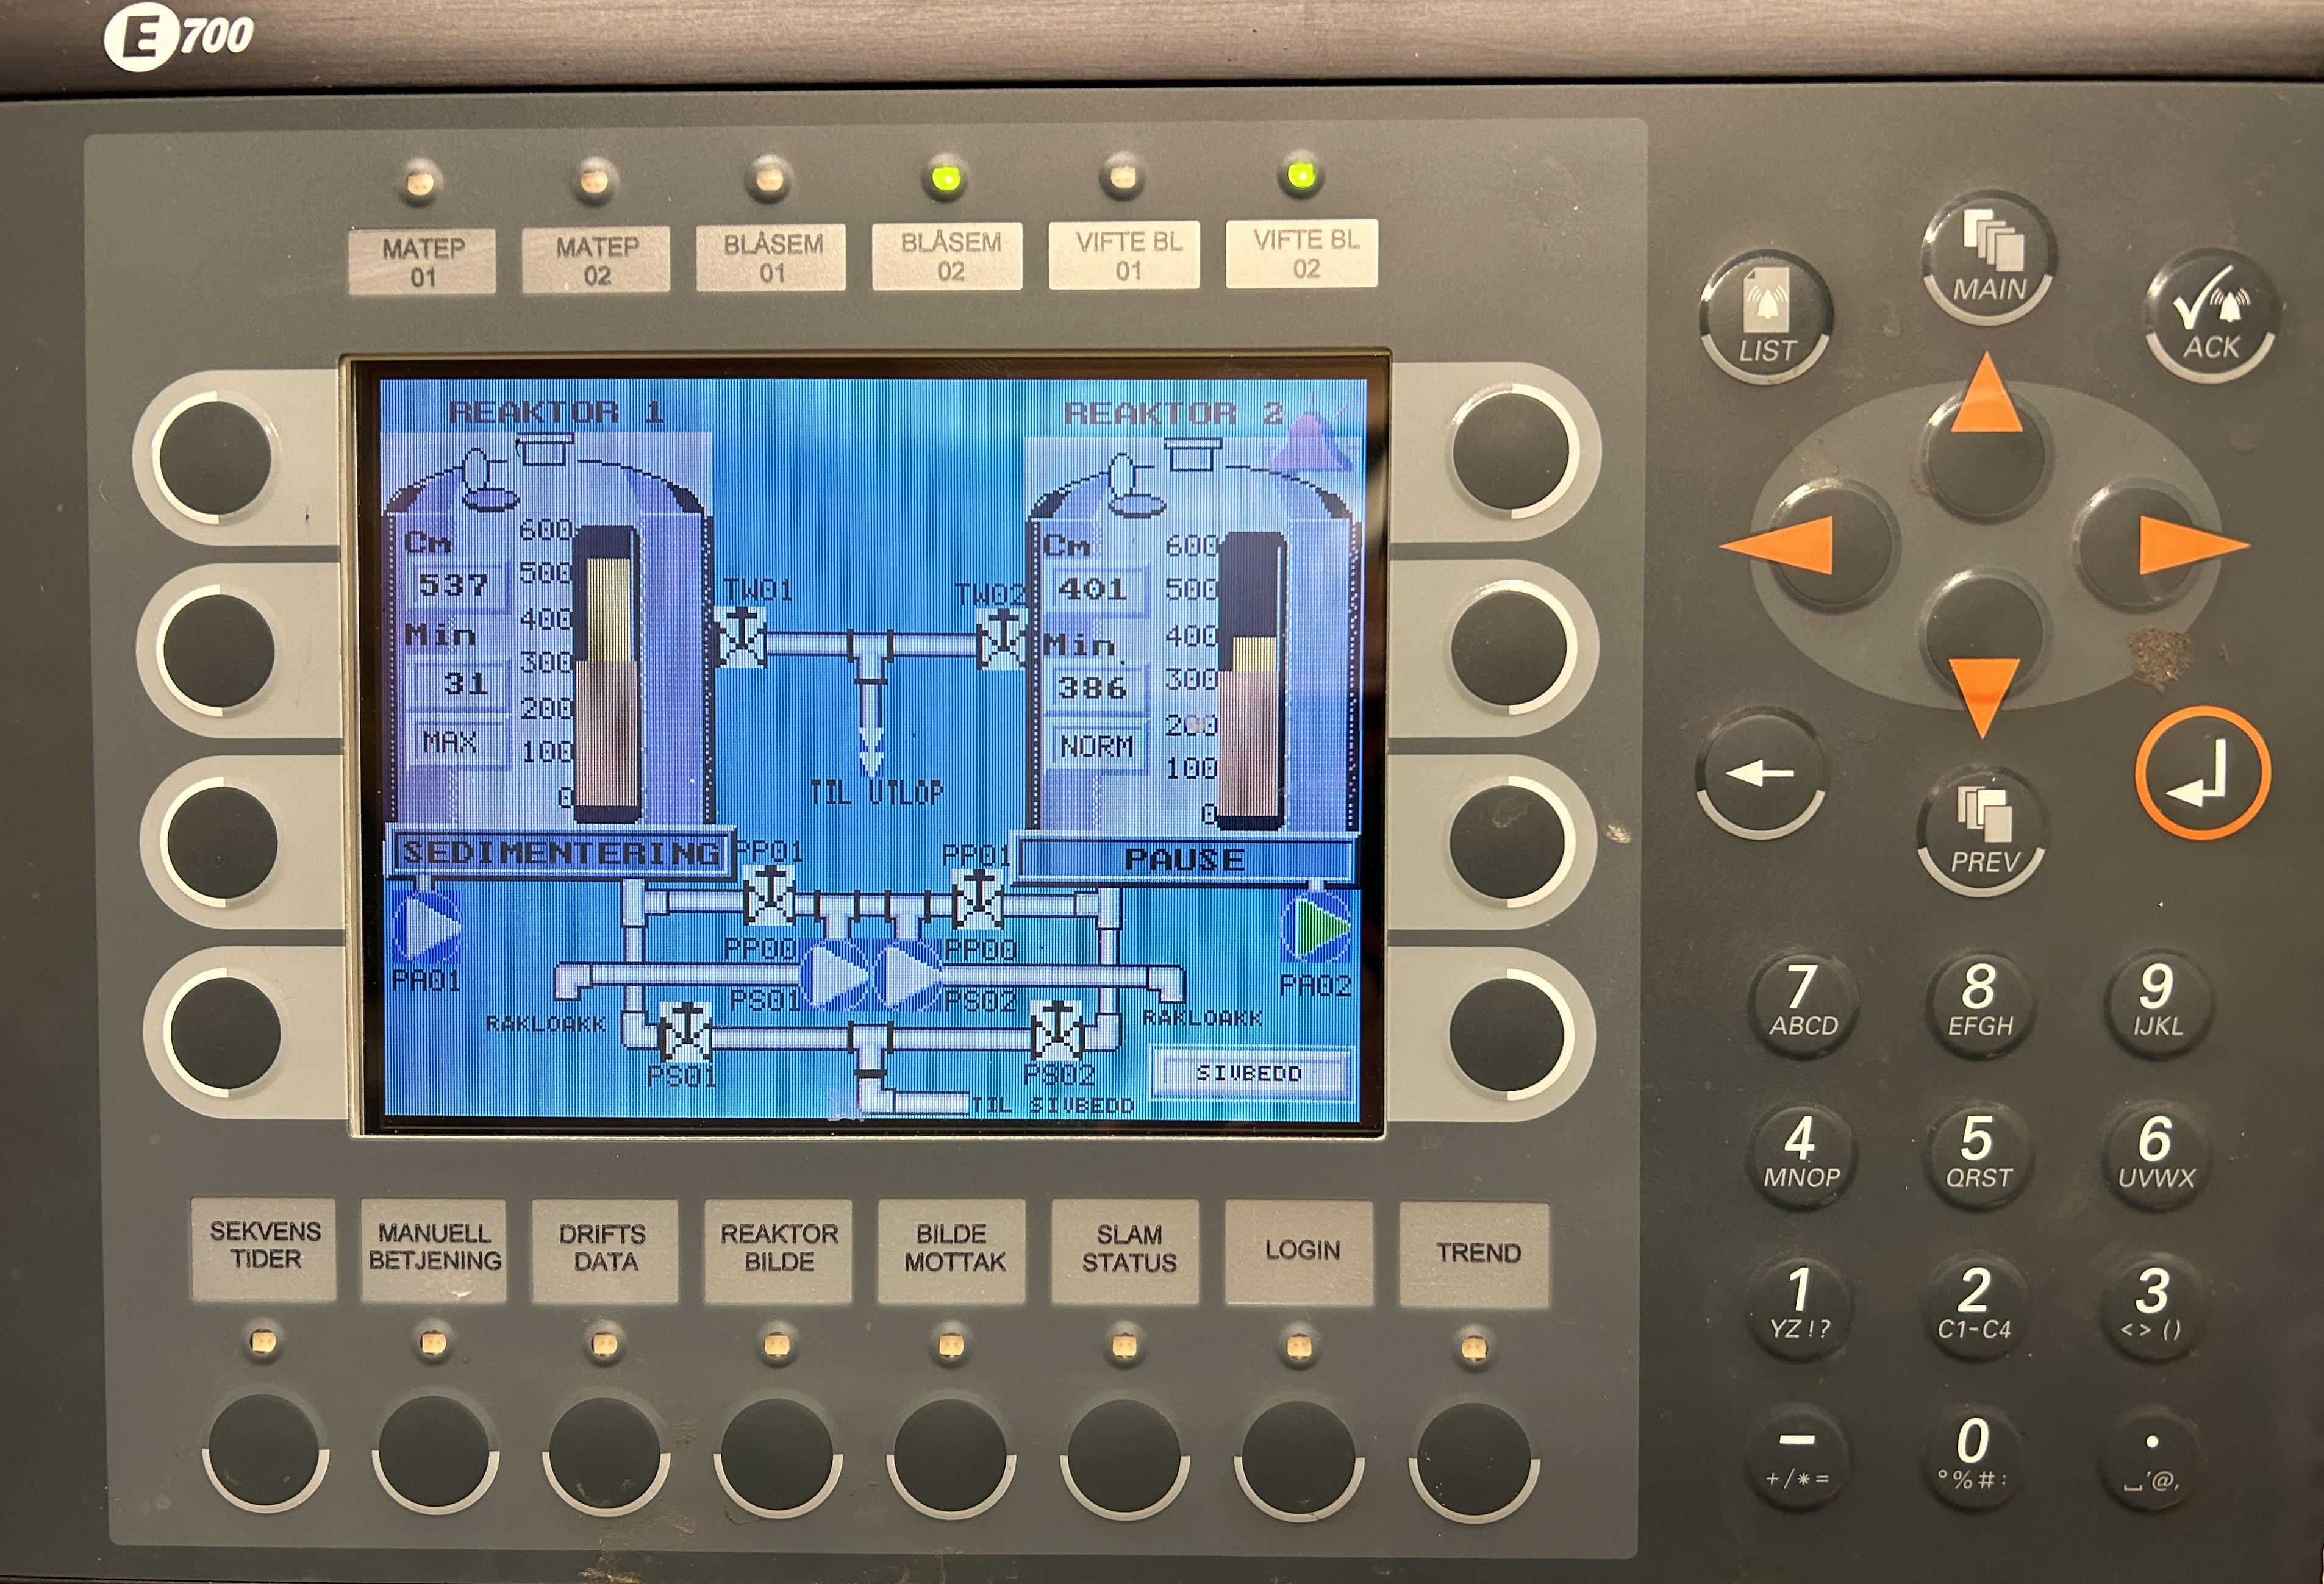
\includegraphics[width=1\textwidth]{Bilder/BeijerSkjerm.JPG}
        \caption{Beijer \gls{HMI}}\label{fig:BeijerSkjerm}
    \end{subfigure}
    \hfill
    \begin{subfigure}[b]{0.3\textwidth}
        \centering
        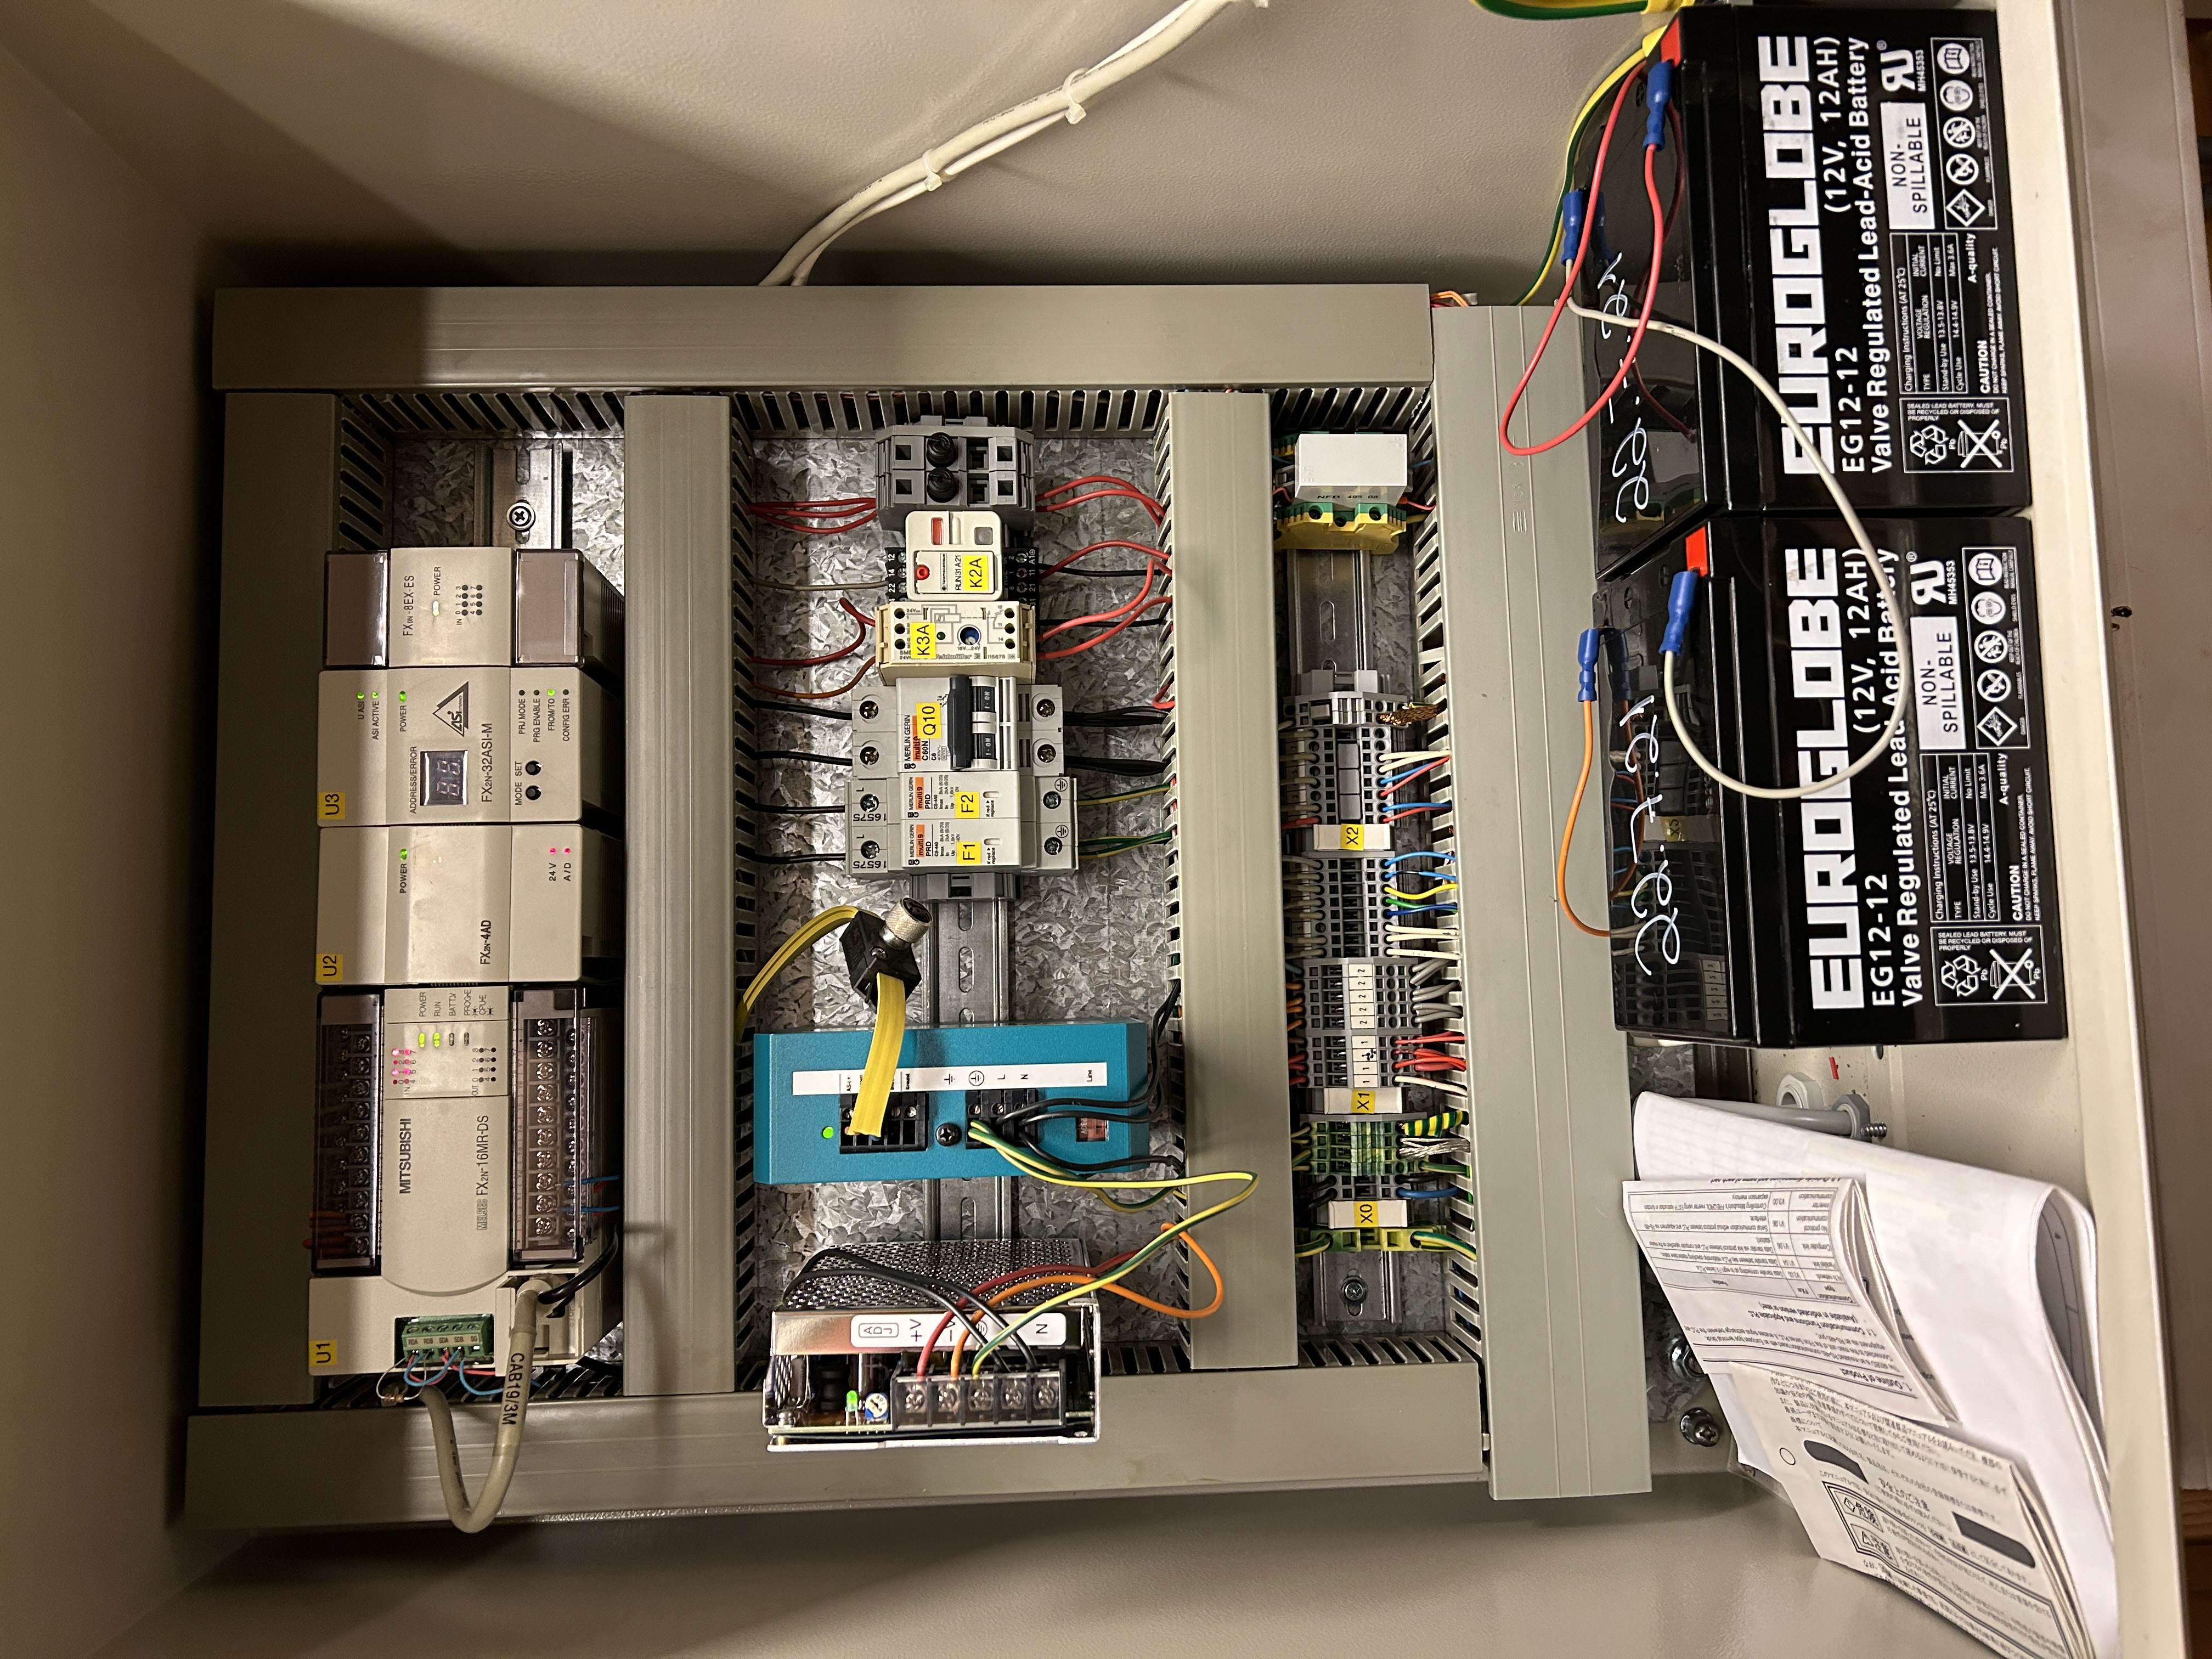
\includegraphics[angle=-90,width=1\textwidth]{Bilder/Styreskap.JPG}
        \caption{Styreskap}\label{fig:Styreskap}
    \end{subfigure}
    \caption{Styresystem}\label{fig:Styresystem}
\end{figure}
